\section{Binary code decimal und 7-Segment Anzeige} % (fold)
\label{sec:Binary code decimal und 7-Segment Anzeige}
\begin{frame}
    \frametitle{BCD und 7-Segment Anzeige}
    \framesubtitle{}
    \begin{figure}[H]
    \begin{center}
            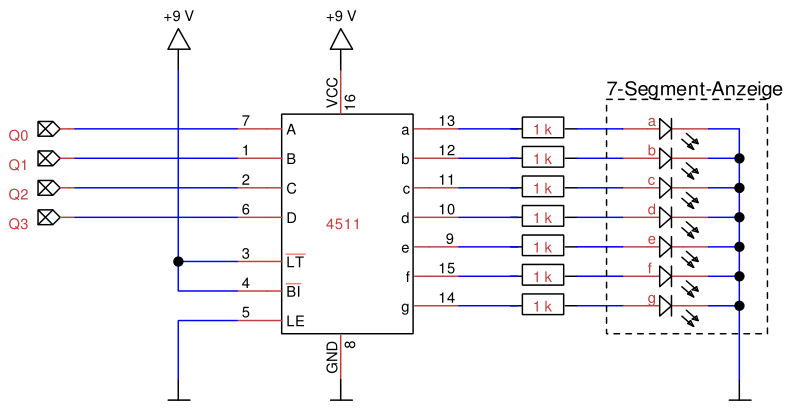
\includegraphics[scale=0.3]{./img/schaltung/bcd.png}
    \end{center}
    \end{figure}
\end{frame}
\begin{frame}
    \frametitle{Funktionsweise}
    \framesubtitle{}
    \begin{columns}[c]
        \column{0.7\textwidth}
            \begin{figure}[H]
                \begin{center}
                        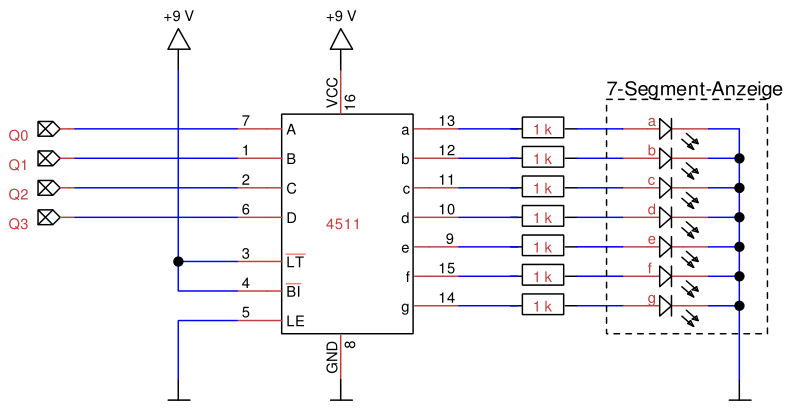
\includegraphics[scale=0.2]{./img/schaltung/bcd.png}
                \end{center}
            \end{figure}
        \column{0.3\textwidth}
            \begin{figure}[H]
            \begin{center}
                    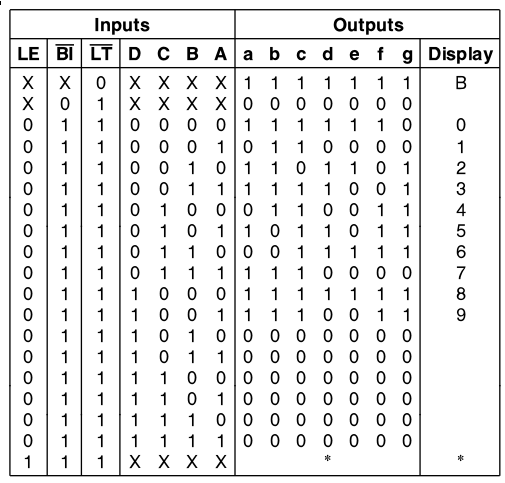
\includegraphics[scale=0.2]{./img/schaltung/sieben_seg.png}
            \end{center}
            \end{figure}
    \end{columns}
    \begin{block}{}
            IC konvertiert 4-bit Nummer in ein
            zur 7-Segment Anzeige passendes Signal
    \end{block}
\end{frame}
\begin{frame}
    \frametitle{Bemerkungen}
    \framesubtitle{}
    \begin{block}{Problem}
         \begin{itemize}
             \item Zähler zählt bis 15, 7-Seg kann aber nur 0-9 anzeigen
             \item größte Zahl ist $(1001)_2 = (9)_{10}$
             \item AND Verbindung von 2. und 4. Bit auf alle Resets "löscht"
             alle Zahlen größer als 9
         \end{itemize}
    \end{block}
    \begin{block}{Würfel}
         \begin{itemize}
             \item Rechtecksspannung kann als Input verwenden werden
             \item hochfrequentiges Zählen wird vom Auge nicht mehr
             wahrgenommen
             \item $\rightarrow$ Psudo-Zufallszahlen
         \end{itemize}
    \end{block}
\end{frame}
% section Binary code decimal und 7-Segment Anzeige (end)
